
\documentclass{beamer}

\usetheme[subsectionpage=progressbar]{metropolis}

\usepackage{tikz}
\usetikzlibrary{babel}
\usetikzlibrary{arrows,shapes,positioning,shadows,trees,calc,fit}
\usetikzlibrary{overlay-beamer-styles} % 'visible on' option for nodes
\usepackage{adjustbox}


\title{Résolution de niveaux du Sokoban}
\date{\today}
\author{PoulpoGaz, darth-mole}
\institute{Candidat n° 012345}

\usepackage{graphics}
\graphicspath{{../../assets/}}
\usepackage{subcaption}

% French language support (e.g. date format)
\usepackage[french]{babel}
\usepackage[T1]{fontenc}
\usepackage{lmodern} % for missing fonts (e.g. italic in titles)

\newenvironment{customtree}{
    \begin{tikzpicture}
        [sibling distance = 10em,
        level distance = 6em,
        every node/.style = {
            shape=rectangle,
            draw,
            scale=0.85
        },
        dot/.style = {
            font = \Large
        },
        edge from parent path = {
            (\tikzparentnode) |-                          % Start from parent
            ($(\tikzparentnode)!0.5!(\tikzchildnode)$) -| % make an ortho line to mid point
            (\tikzchildnode)                              % make another ortho to the target
        }
    ]
}{
    \end{tikzpicture}%
}

\begin{document}

    \maketitle

    \begin{frame}{Plan}
        \tableofcontents%[hideallsubsections]
    \end{frame}

    \section{Le jeu du Sokoban}
        \begin{frame}{Le jeu du Sokoban}
            \begin{columns}
                \begin{column}{0.3\textwidth}
                    \begin{figure}
                        \centering
                        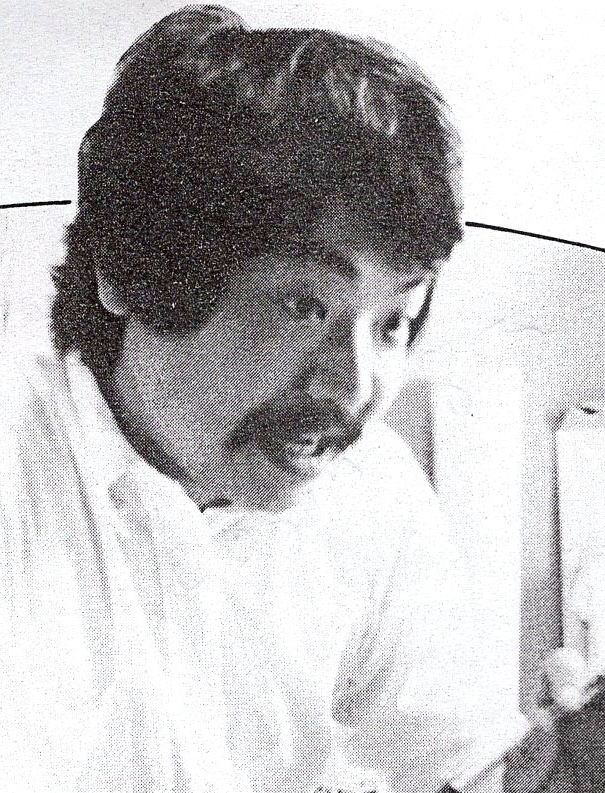
\includegraphics[width=\columnwidth]{creator.jpg}
                        \caption*{Hiroyuki Imabayashi}
                    \end{figure}
                \end{column}
                \begin{column}{0.7\textwidth}
                    \begin{figure}
                        \centering
                        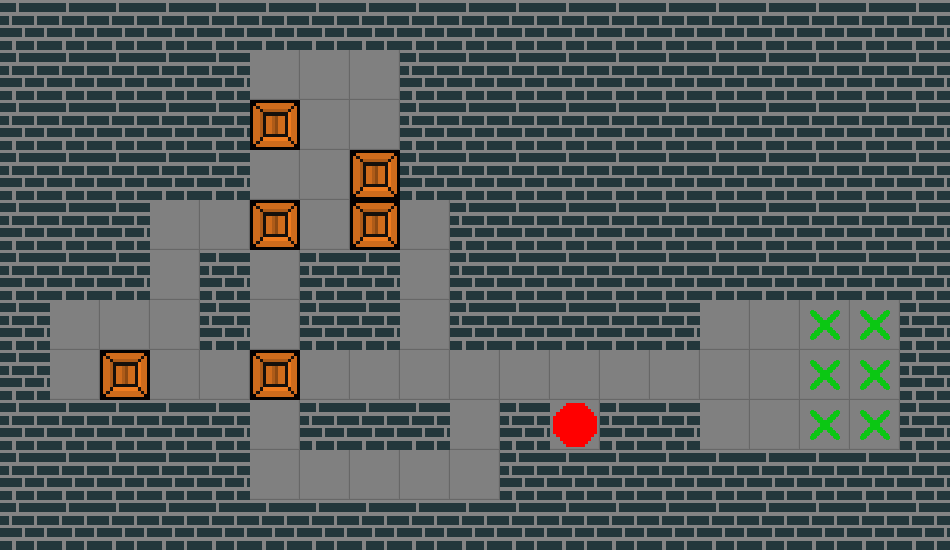
\includegraphics[width=\columnwidth]{level_example.png}
                        \caption*{\textit{XSokoban}}
                    \end{figure}
                \end{column}
            \end{columns}
        \end{frame}

        \begin{frame}{But du jeu}
            \centering
            \resizebox{\textwidth}{!}{%
                \begin{tikzpicture}
                    \node (start) {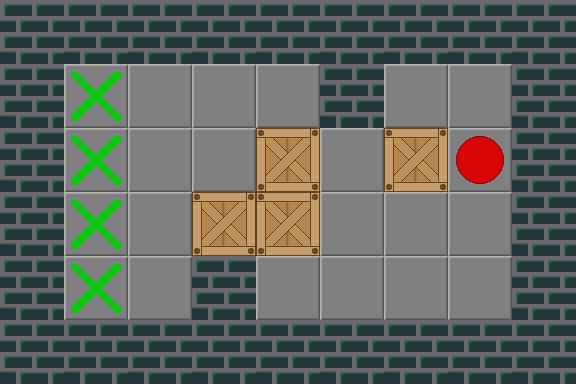
\includegraphics[width=0.5\textwidth]{rules/game_start.png}};
                    \node (end) [right=of start]{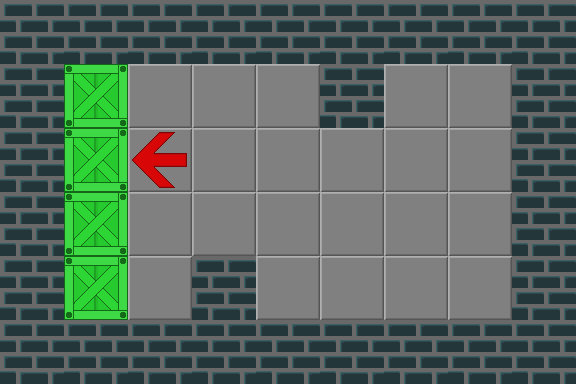
\includegraphics[width=0.5\textwidth]{rules/game_end.png}};
                    \draw[->, line width=1mm] (start.north east) to[out=60,in=130] node (label) [anchor=south, midway] {Déplacements} (end.north west);
                \end{tikzpicture}
            }
        \end{frame}

        \begin{frame}{Règles}
            \begin{columns}\usetikzlibrary{shadows,shapes,positioning}
                \begin{column}{0.5\textwidth}
                    \only<1-2>{
                        \begin{figure}
                            \centering
                            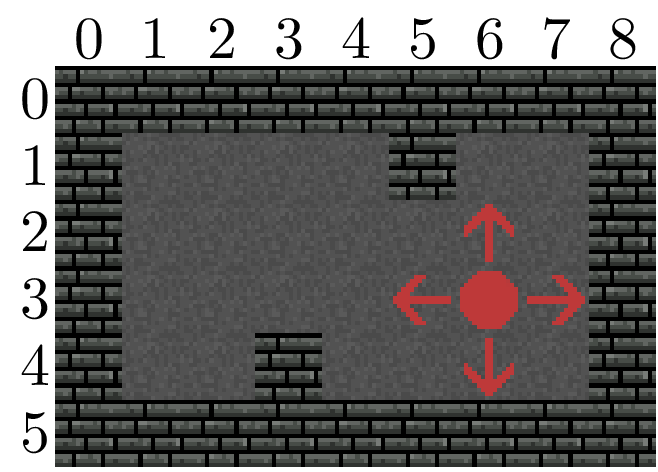
\includegraphics[width=0.9\textwidth]{rules/moves.png}
                            \caption*{Déplacements autorisés}
                        \end{figure}
                    }
                    \only<3>{
                        \begin{figure}
                            \centering
                            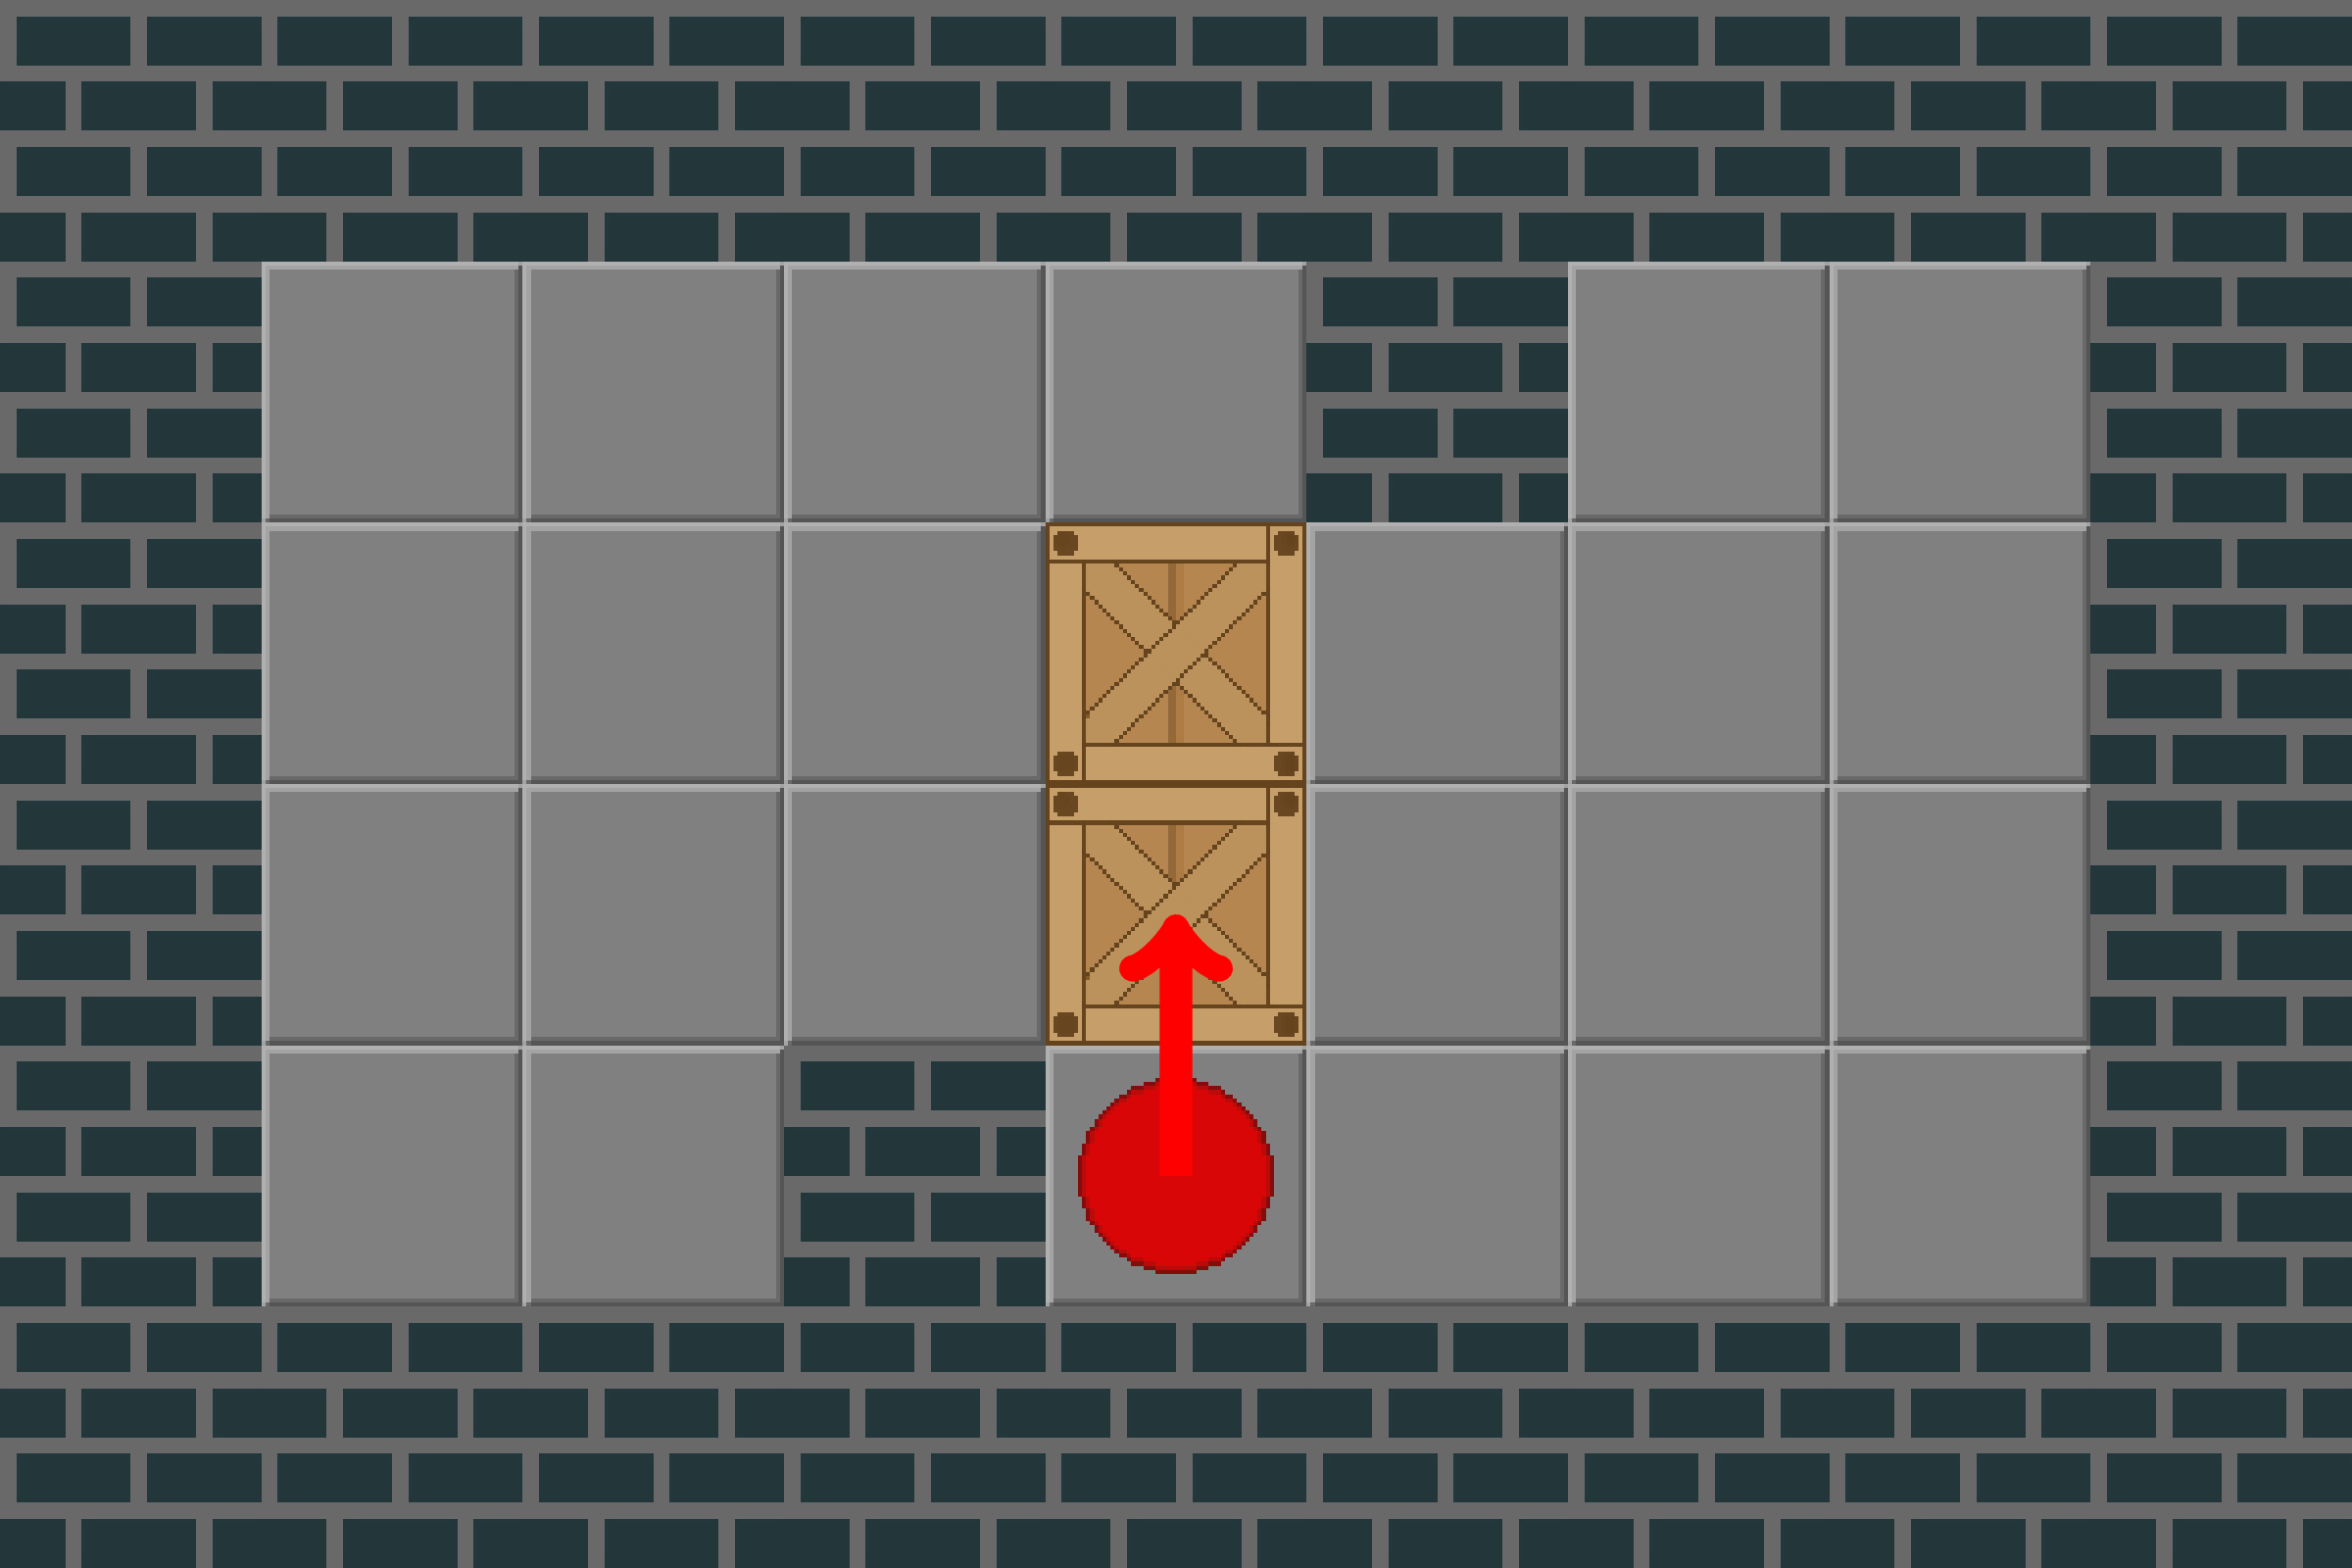
\includegraphics[width=0.9\textwidth]{rules/move_no_1.png}
                            \caption*{
\includegraphics[width=\iconwidth]{icons/no.png}}
                        \end{figure}
                    }
                \end{column}
                \begin{column}{0.5\textwidth}
                    \only<2>{
                        \begin{figure}
                            \centering
                            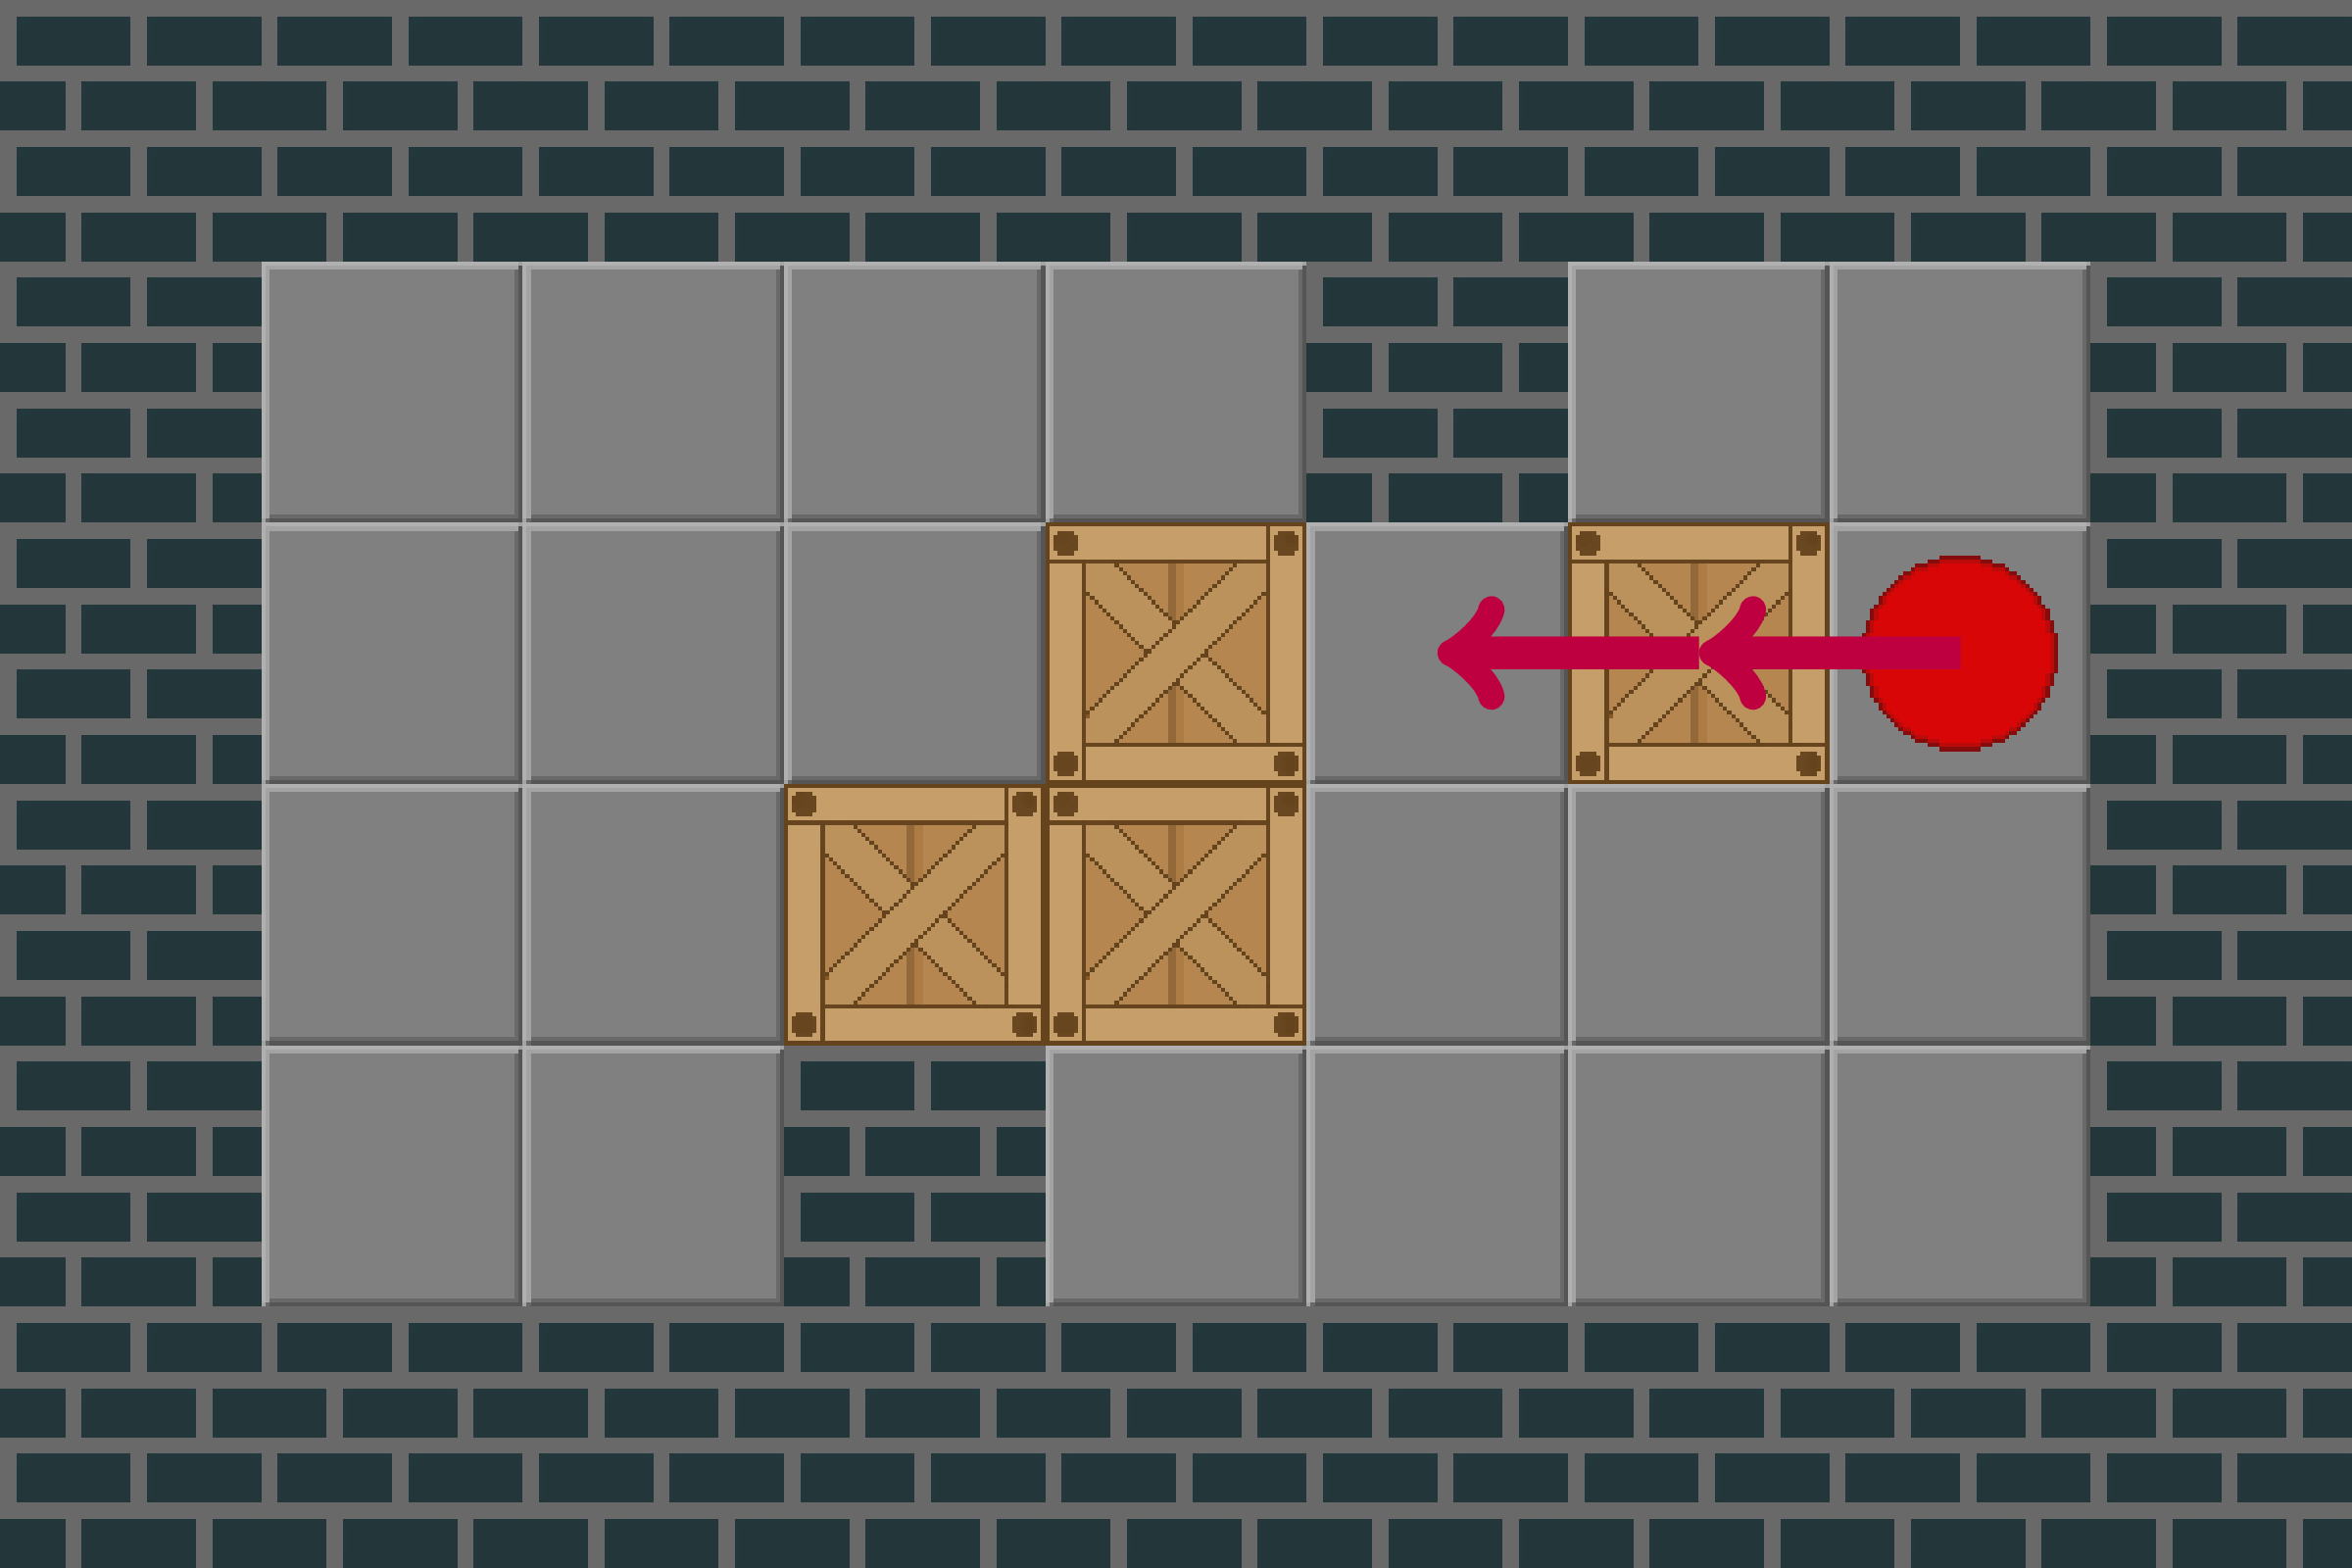
\includegraphics[width=0.9\textwidth]{rules/move_yes.png}
                            \caption*{
\includegraphics[width=\iconwidth]{icons/yes.png}}
                        \end{figure}
                    }
                    \only<3>{
                        \begin{figure}
                            \centering
                            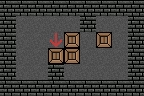
\includegraphics[width=0.9\textwidth]{rules/move_no_2.png}
                            \caption*{
\includegraphics[width=\iconwidth]{icons/no.png}}
                        \end{figure}
                    }
                \end{column}
            \end{columns}
        \end{frame}

        \begin{frame}{Tuiles} 
            \centering

            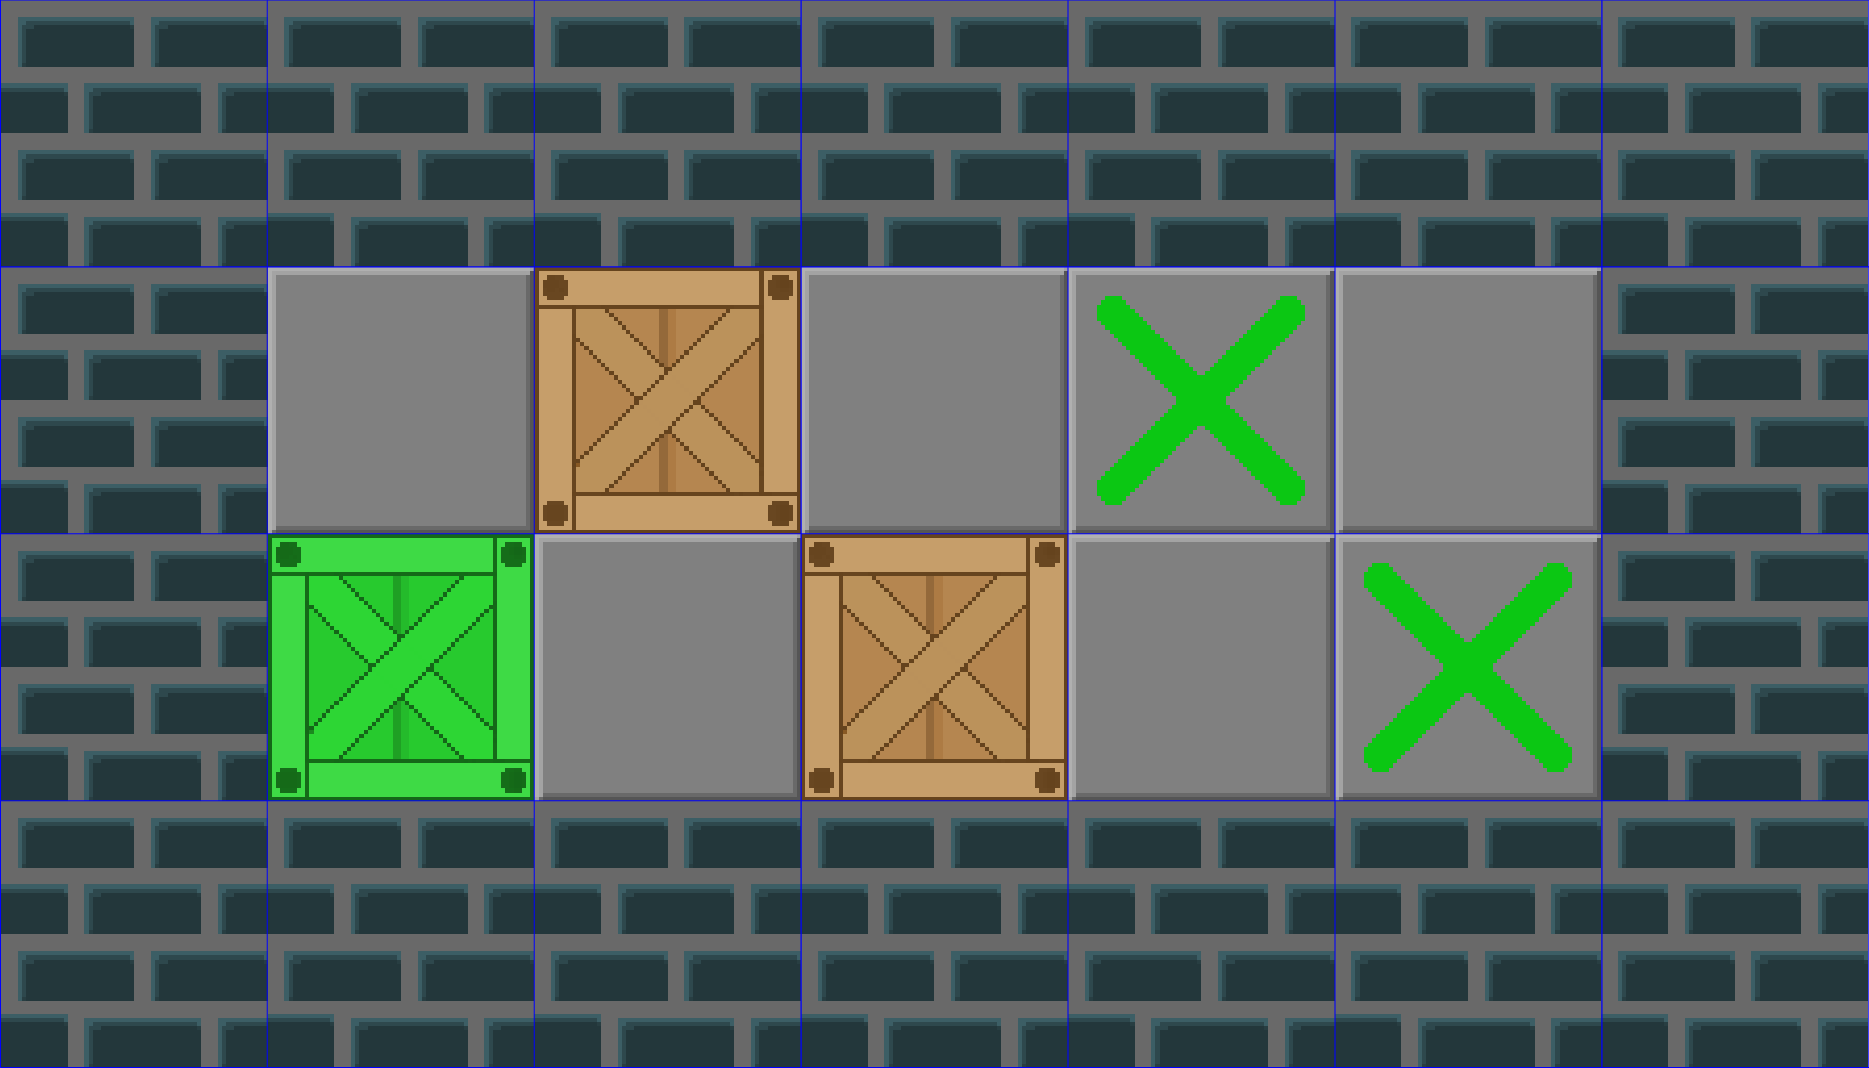
\includegraphics[width=0.5\textwidth]{tiles/tilemap.png}

            \resizebox{\textwidth}{!}{%
                \begin{tabular}{ c c c c c }
                    
\includegraphics[width=0.2\textwidth]{tiles/wall.png} &
                    
\includegraphics[width=0.2\textwidth]{tiles/floor.png} &
                    
\includegraphics[width=0.2\textwidth]{tiles/crate.png} &
                    
\includegraphics[width=0.2\textwidth]{tiles/target.png} &
                    
\includegraphics[width=0.2\textwidth]{tiles/crate_on_target.png} \\
                   \textbf{Mur} & Sol & \textbf{Caisse} & Cible & \textbf{Caisse sur une cible} \\
                \end{tabular}
            }

            % For some reason, the minted environement is not working
            \only<2>{
                \mint{java}|enum Tile {WALL, FLOOR, CRATE, TARGET, CRATE_ON_TARGET};|
                \mint{java}|Tile[][] map = new Tile[height][width];|
            }
           
        \end{frame}

        \begin{frame}{Lien avec le thème de l'année}
            \centering
            \only<1>{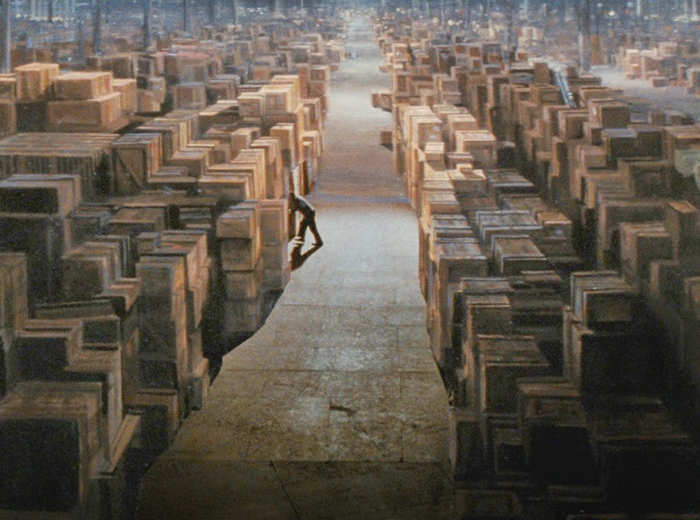
\includegraphics[width=0.9\textwidth]{warehouse.jpg}}
            \only<2>{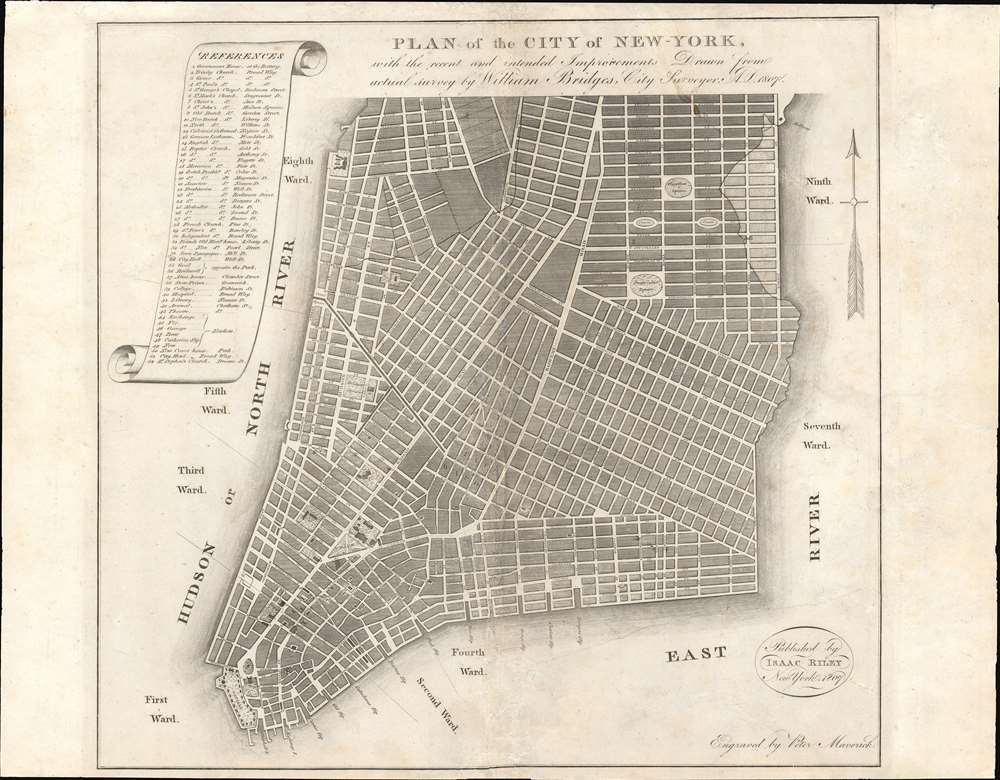
\includegraphics[width=0.9\textwidth]{city_plan.jpg}}
        \end{frame}

    \section{Principe de résolution}
            \begin{frame}{Arbre des états}
                \begin{customtree}
                    
\node{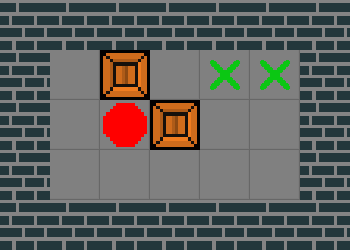
\includegraphics[width=0.3\textwidth]{exhaustive_search/1.png}}
child[visible on=<2->]{
    node{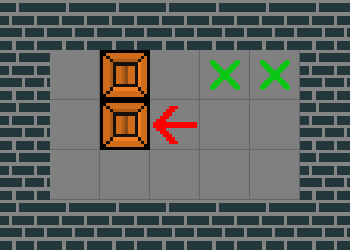
\includegraphics[width=0.3\textwidth]{exhaustive_search/1_1.png}}
    child[visible on=<4->]{
        node{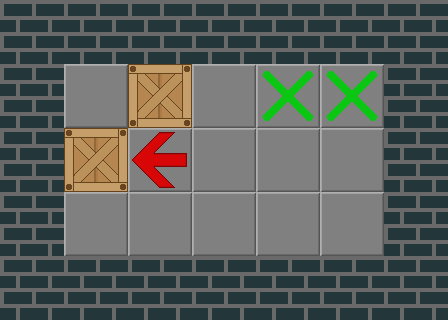
\includegraphics[width=0.3\textwidth]{exhaustive_search/1_1_1.png}}
        child[visible on=<7->]{
            node[dot]{$\dots$}
        }
    } child[visible on=<5->]{
        node{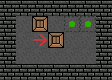
\includegraphics[width=0.3\textwidth]{exhaustive_search/1_1_2.png}}
        child[visible on=<7->]{
            node[dot]{$\dots$}
        }
    }
} child[visible on=<3->]{
    node{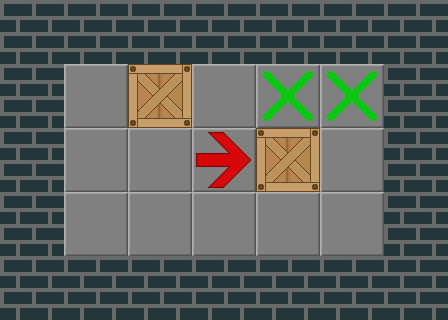
\includegraphics[width=0.3\textwidth]{exhaustive_search/1_2.png}}
    child[visible on=<6->]{
        node[dot]{$\dots$}
    }
};
                \end{customtree}
            \end{frame}

            \begin{frame}{Exemple développé}
                \begin{customtree}
                    \node{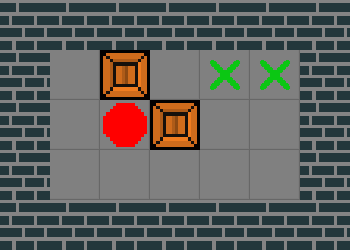
\includegraphics{exhaustive_search/1.png}}
child{
    node{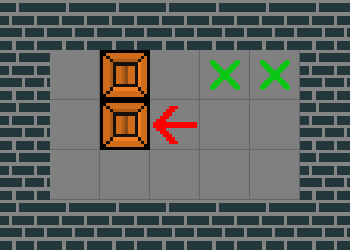
\includegraphics{exhaustive_search/1_1.png}}
    child{
        node{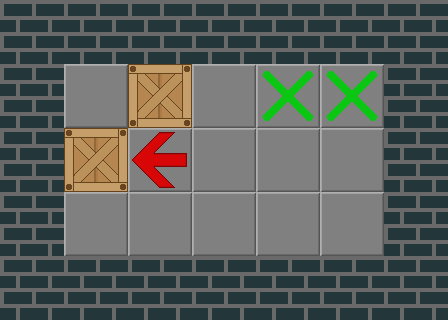
\includegraphics{exhaustive_search/1_1_1.png}}
        child{
            node[dot]{$\dots$}
        }
    } child {
        node{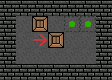
\includegraphics{exhaustive_search/1_1_2.png}}
        child{
            node(sameState1){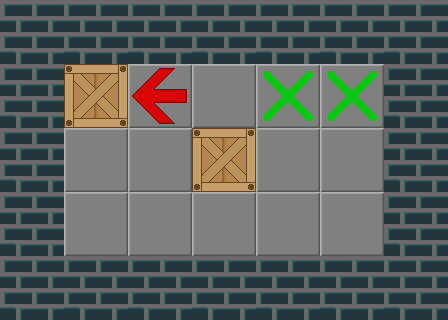
\includegraphics{exhaustive_search/1_1_2_1.png}}
            child{
                node[dot]{$\dots$}
            }
        } child{
            node(sameState2){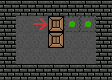
\includegraphics{exhaustive_search/1_1_2_2.png}}
            child{
                node[dot]{$\dots$}
            }
        }
    }
} child{
    node{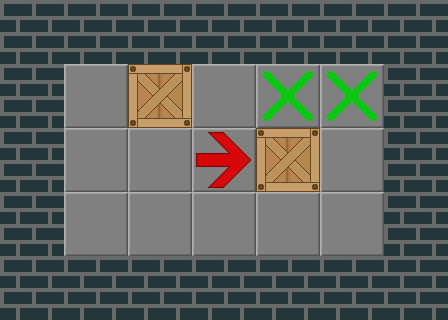
\includegraphics{exhaustive_search/1_2.png}}
    child{
        node[dot]{$\dots$}
    }
} child{
    node(sameState12){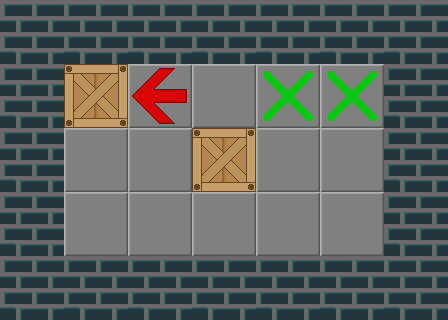
\includegraphics{exhaustive_search/1_3.png}}
    child{
        node[dot]{$\dots$}
    }
} child{
    node(sameState22){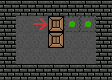
\includegraphics{exhaustive_search/1_4.png}}
    child{
        node[dot]{$\dots$}
    }
};

                    % Put it but not draw it to have the same width on the next slide
                    \node(c22)[ellipse, minimum width=4.2cm, minimum height=3.2cm, line width=1mm, red] at (sameState22.center){};
                \end{customtree}
            \end{frame}

            \begin{frame}{Un graphe vu comme un arbre}
                \begin{customtree}
                    \node{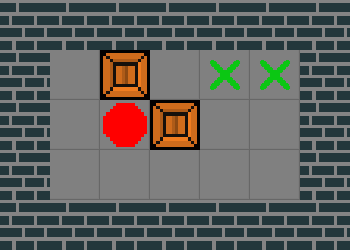
\includegraphics{exhaustive_search/1.png}}
child{
    node{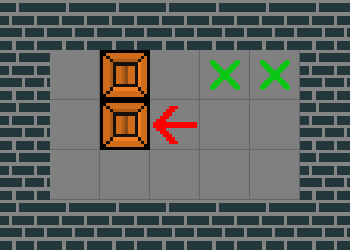
\includegraphics{exhaustive_search/1_1.png}}
    child{
        node{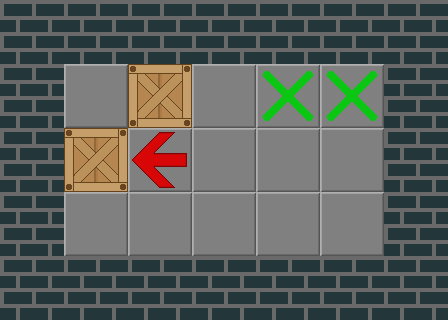
\includegraphics{exhaustive_search/1_1_1.png}}
        child{
            node[dot]{$\dots$}
        }
    } child {
        node{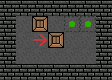
\includegraphics{exhaustive_search/1_1_2.png}}
        child{
            node(sameState1){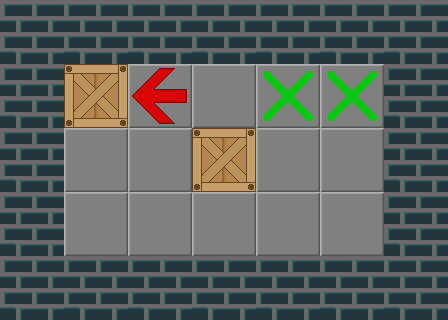
\includegraphics{exhaustive_search/1_1_2_1.png}}
            child{
                node[dot]{$\dots$}
            }
        } child{
            node(sameState2){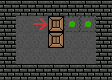
\includegraphics{exhaustive_search/1_1_2_2.png}}
            child{
                node[dot]{$\dots$}
            }
        }
    }
} child{
    node{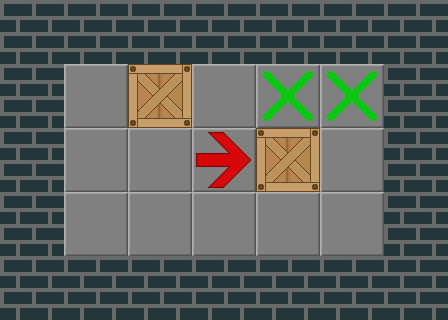
\includegraphics{exhaustive_search/1_2.png}}
    child{
        node[dot]{$\dots$}
    }
} child{
    node(sameState12){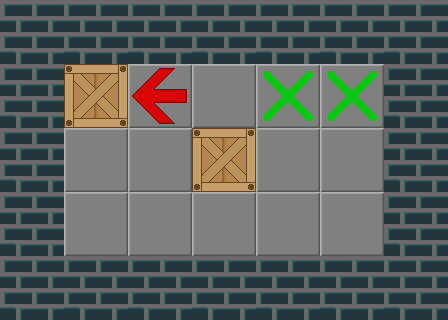
\includegraphics{exhaustive_search/1_3.png}}
    child{
        node[dot]{$\dots$}
    }
} child{
    node(sameState22){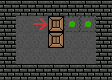
\includegraphics{exhaustive_search/1_4.png}}
    child{
        node[dot]{$\dots$}
    }
};

                    \node(c1)[draw, ellipse, minimum width=4.2cm, minimum height=3.2cm, line width=1mm, red] at (sameState1.center){};
                    \node(c2)[draw, ellipse, minimum width=4.2cm, minimum height=3.2cm, line width=1mm, red] at (sameState2.center){};
                    \node(c12)[draw, ellipse, minimum width=4.2cm, minimum height=3.2cm, line width=1mm, red] at (sameState12.center){};
                    \node(c22)[draw, ellipse, minimum width=4.2cm, minimum height=3.2cm, line width=1mm, red] at (sameState22.center){};

                    \draw[<->, draw=red, line width = 2mm] (c1.north) |- (c12.west);
                    \draw[<->, draw=red, line width = 2mm] (c2.east) -| (c22.south);
                \end{customtree}
            \end{frame}

    \section{Réduction de l'espace de recherche}

        \subsection{Analyse statique}

            \begin{frame}{Détection des positions mortes \textit{(dead positions)}}
                \centering
                \only<1>{
                    \begin{tikzpicture}
                        \node(before){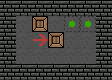
\includegraphics{dead_positions/example_before.png}};
                        \node(after)[right=of before]{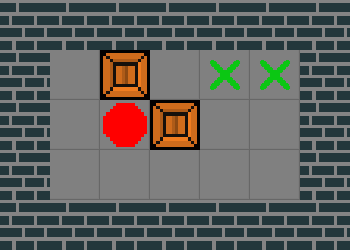
\includegraphics{dead_positions/example_after.png}};
                        \draw[->, line width=\arrowwidth] (before) -- (after);
                    \end{tikzpicture}
                }
                \only<2-> {
                    \begin{enumerate}
                        \only<2>{
                            \item
                                \begin{tikzpicture}[baseline]
                                    \node(first){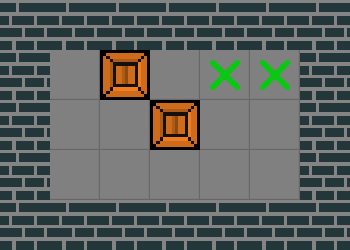
\includegraphics{dead_positions/algo_1_1.png}};
                                    \node(second)[right=of first]{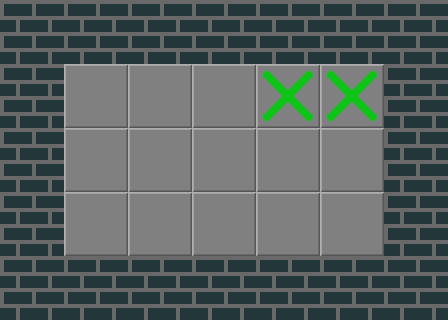
\includegraphics{dead_positions/algo_1_2.png}};
                                    \draw[->, line width=\arrowwidth] (before) -- (after);
                                \end{tikzpicture}
                        }
                        \only<3->{
                            \setcounter{enumi}{1}
                            \item
                                \begin{tikzpicture}[baseline, every node/.style={node distance=0.1cm}]
                                    \node(first){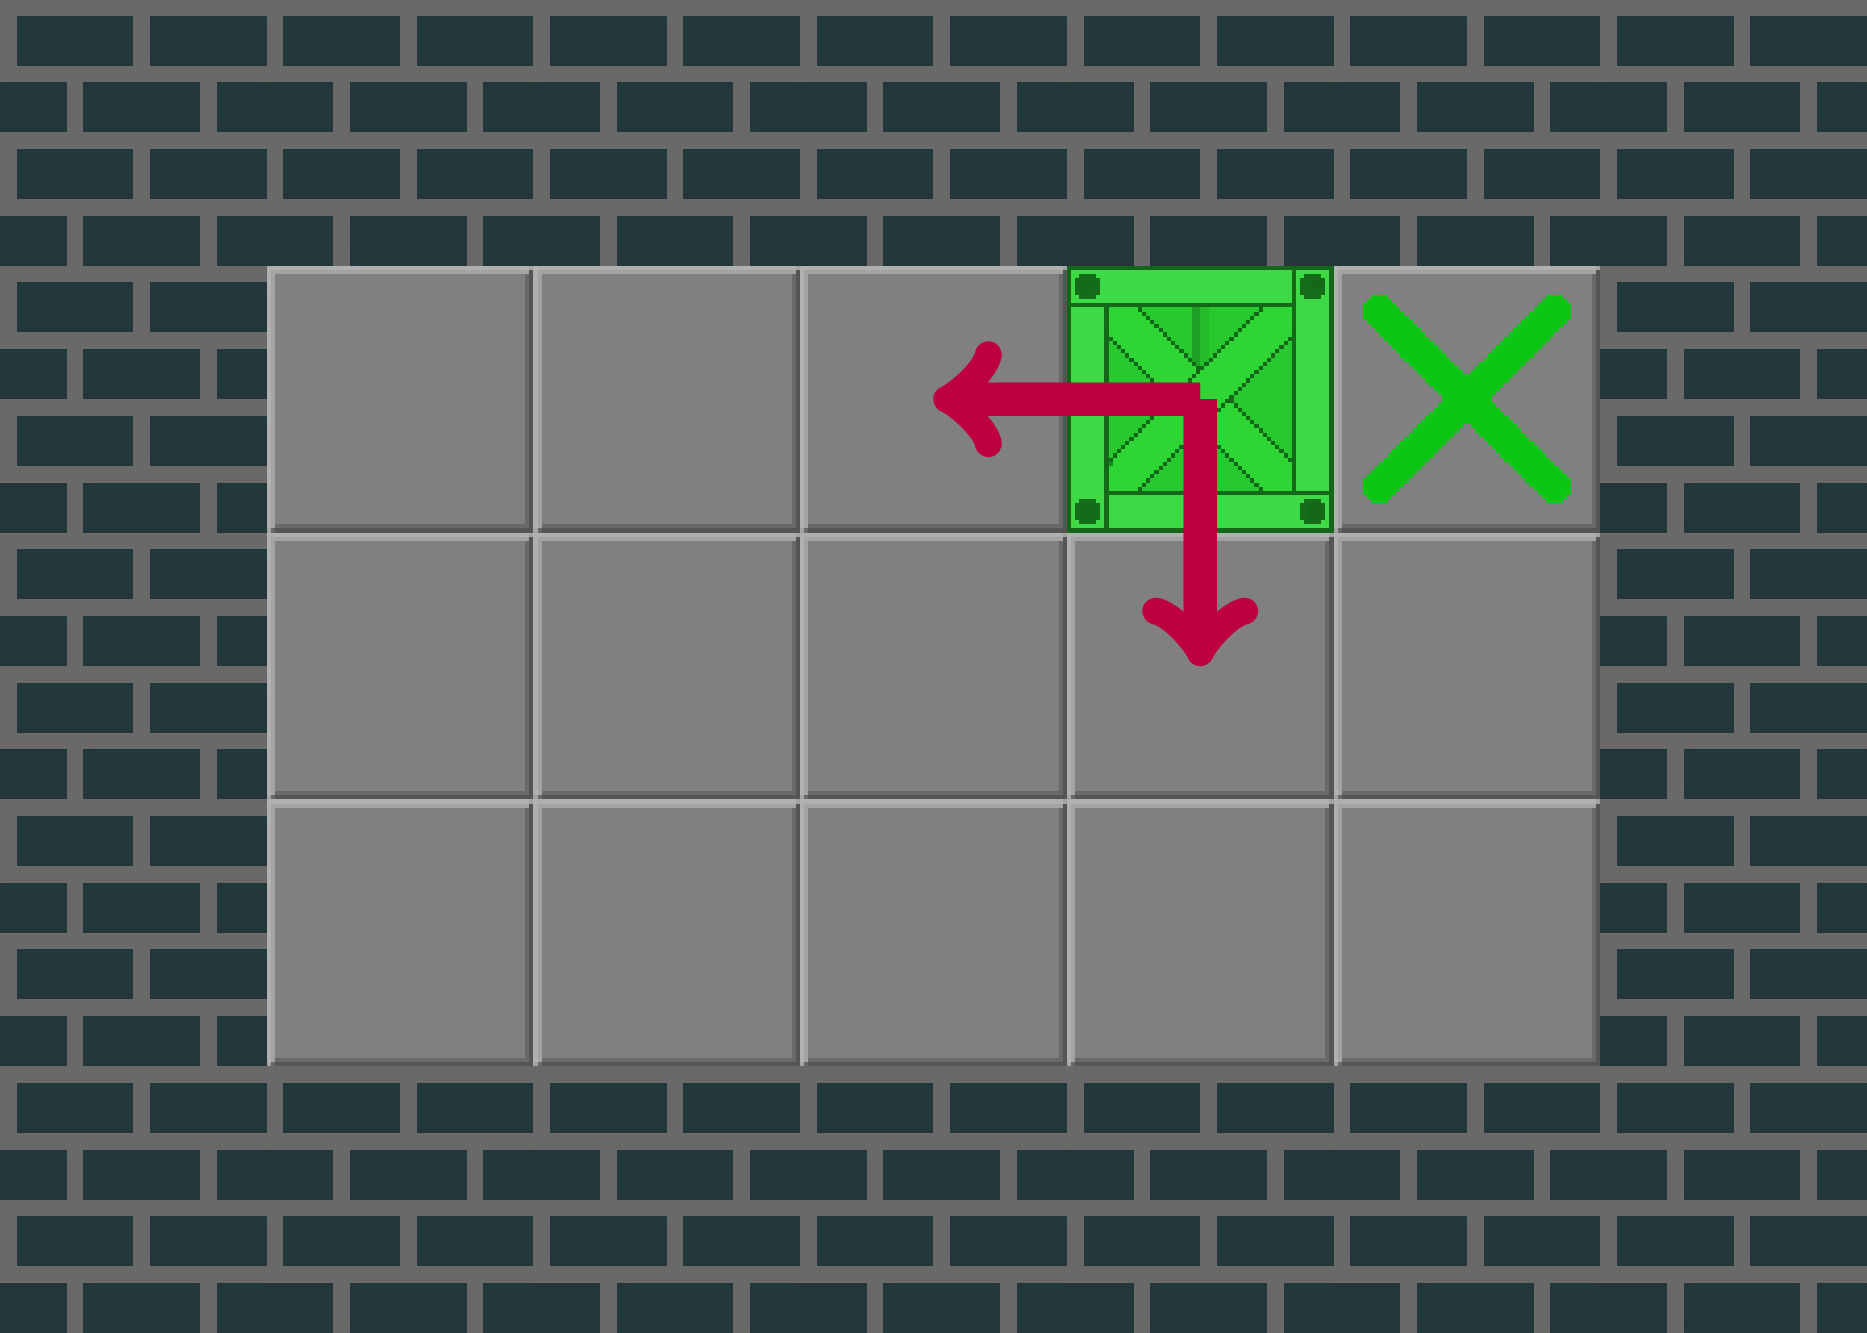
\includegraphics{dead_positions/algo_2_1.png}};
                                    \node(second)[right=of first, visible on=<4>]{$\dots$};
                                    \node[right=of second, visible on=<4>]{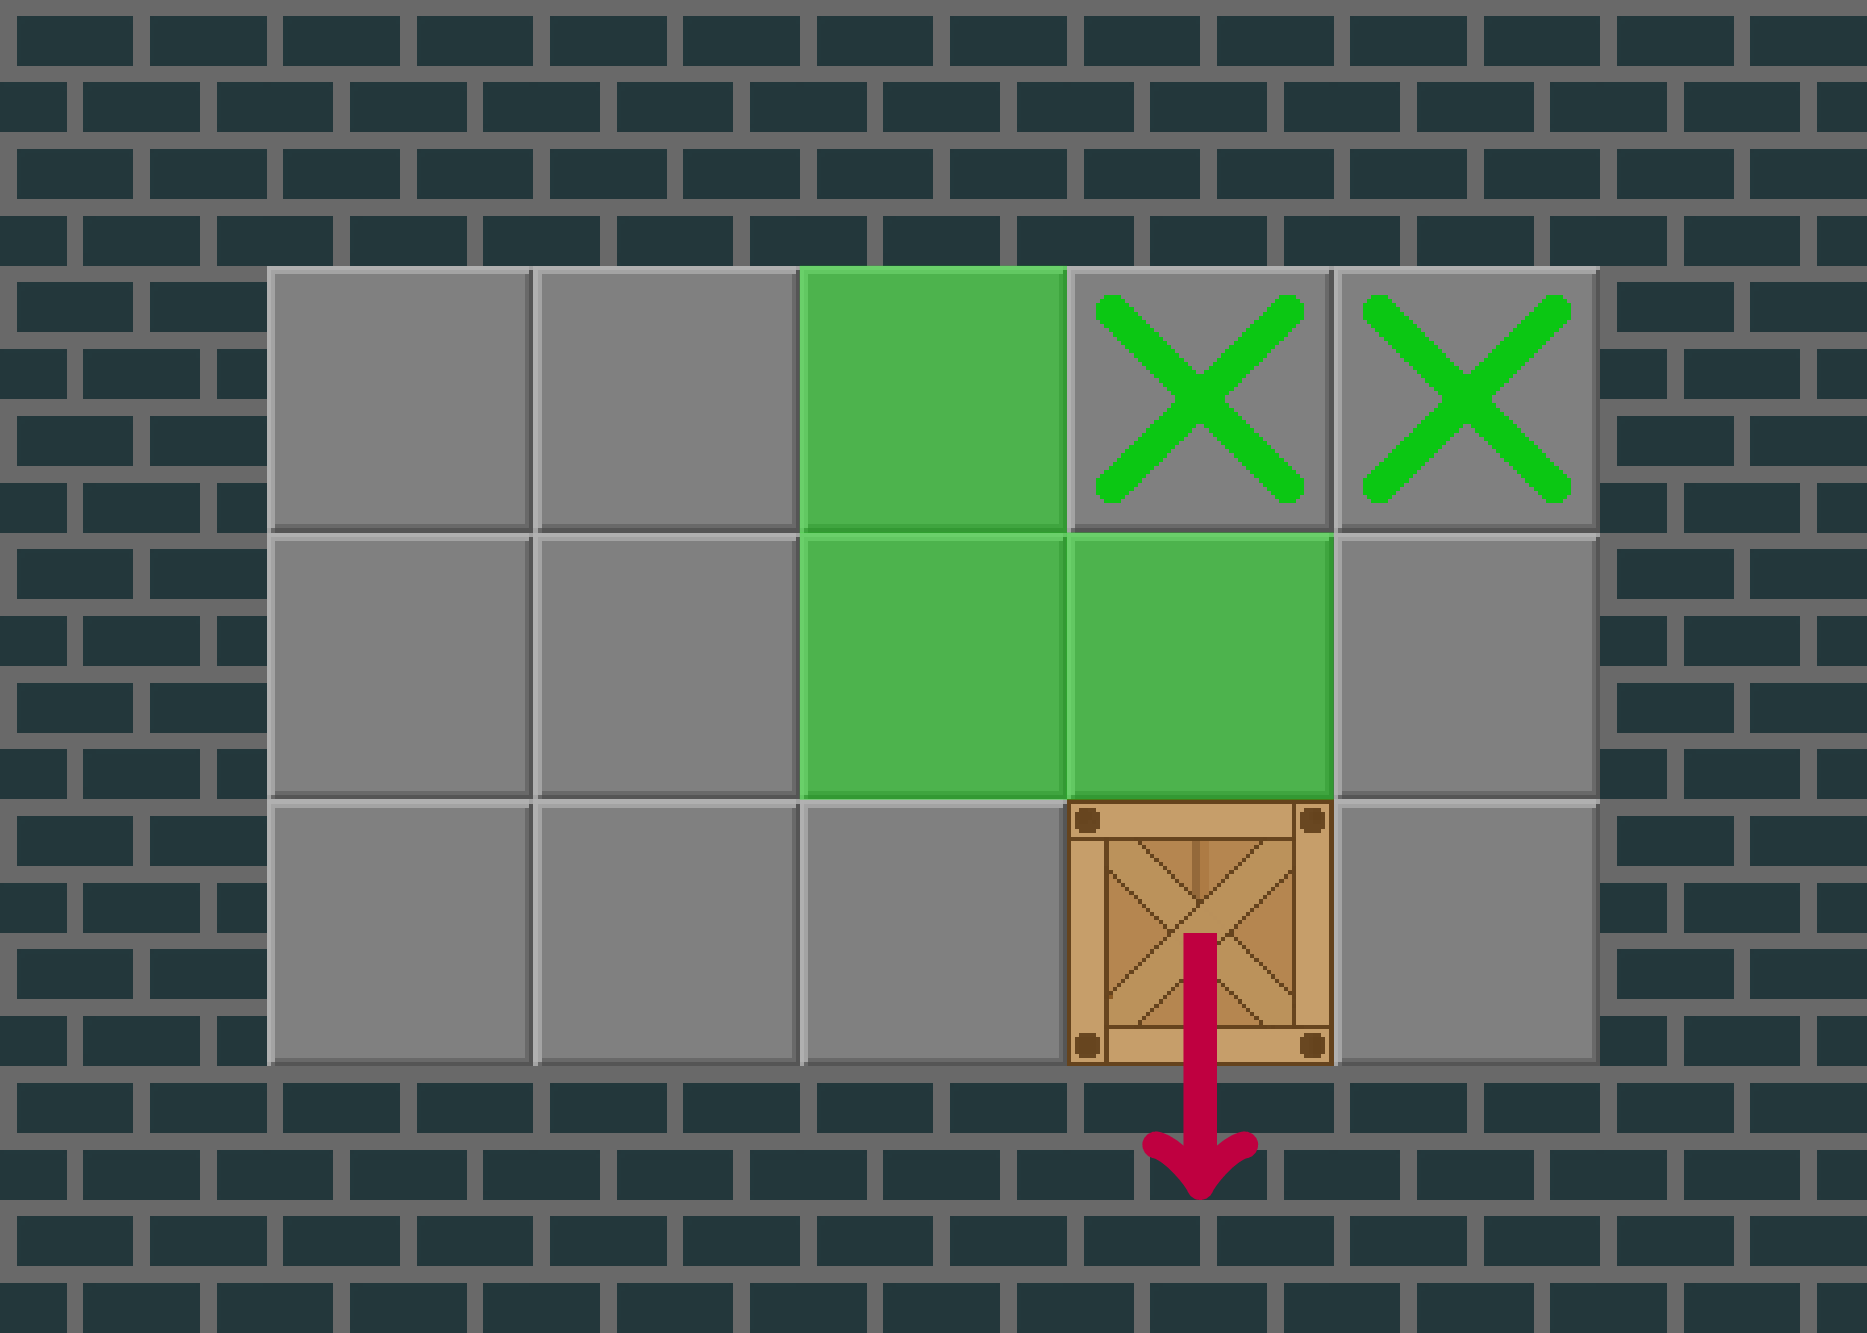
\includegraphics{dead_positions/algo_2_2.png}};
                                \end{tikzpicture}
                        }
                    \end{enumerate}
                }
            \end{frame}

            \begin{frame}{Détection de tunnels}
                \only<1>{
                    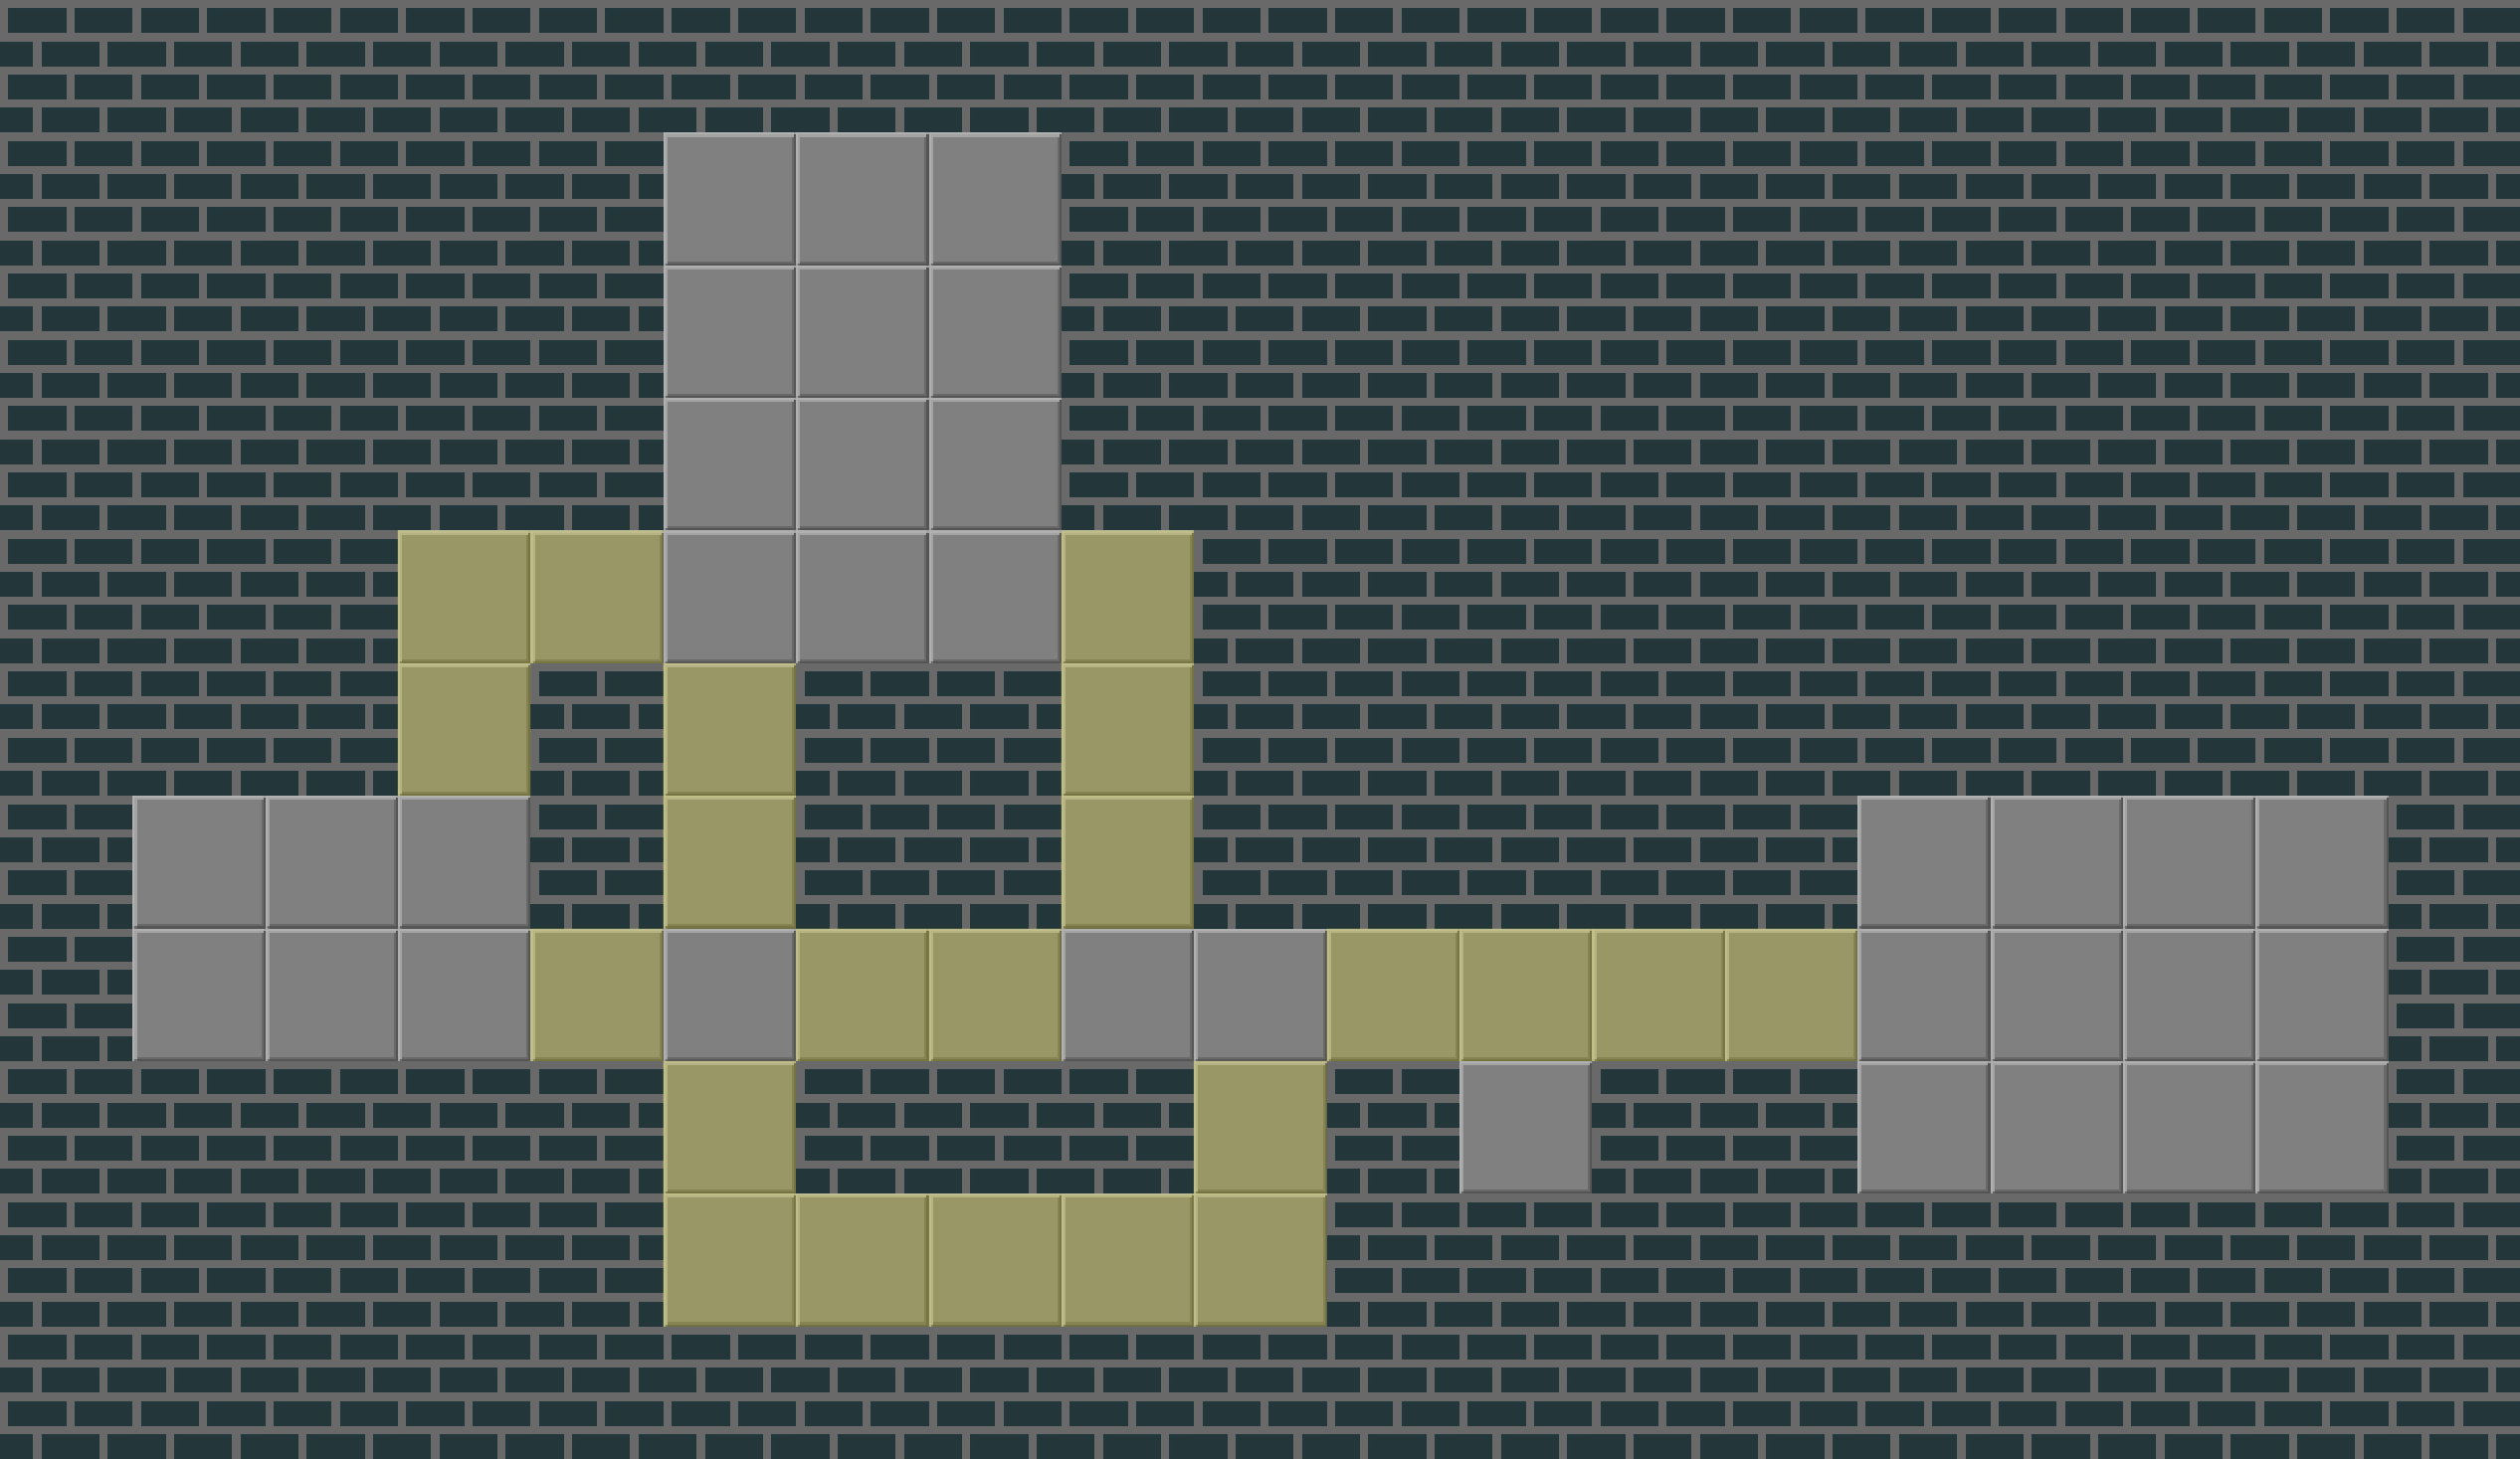
\includegraphics[width=\textwidth]{tunnels/tunnels.png}
                }
                \only<2>{
                     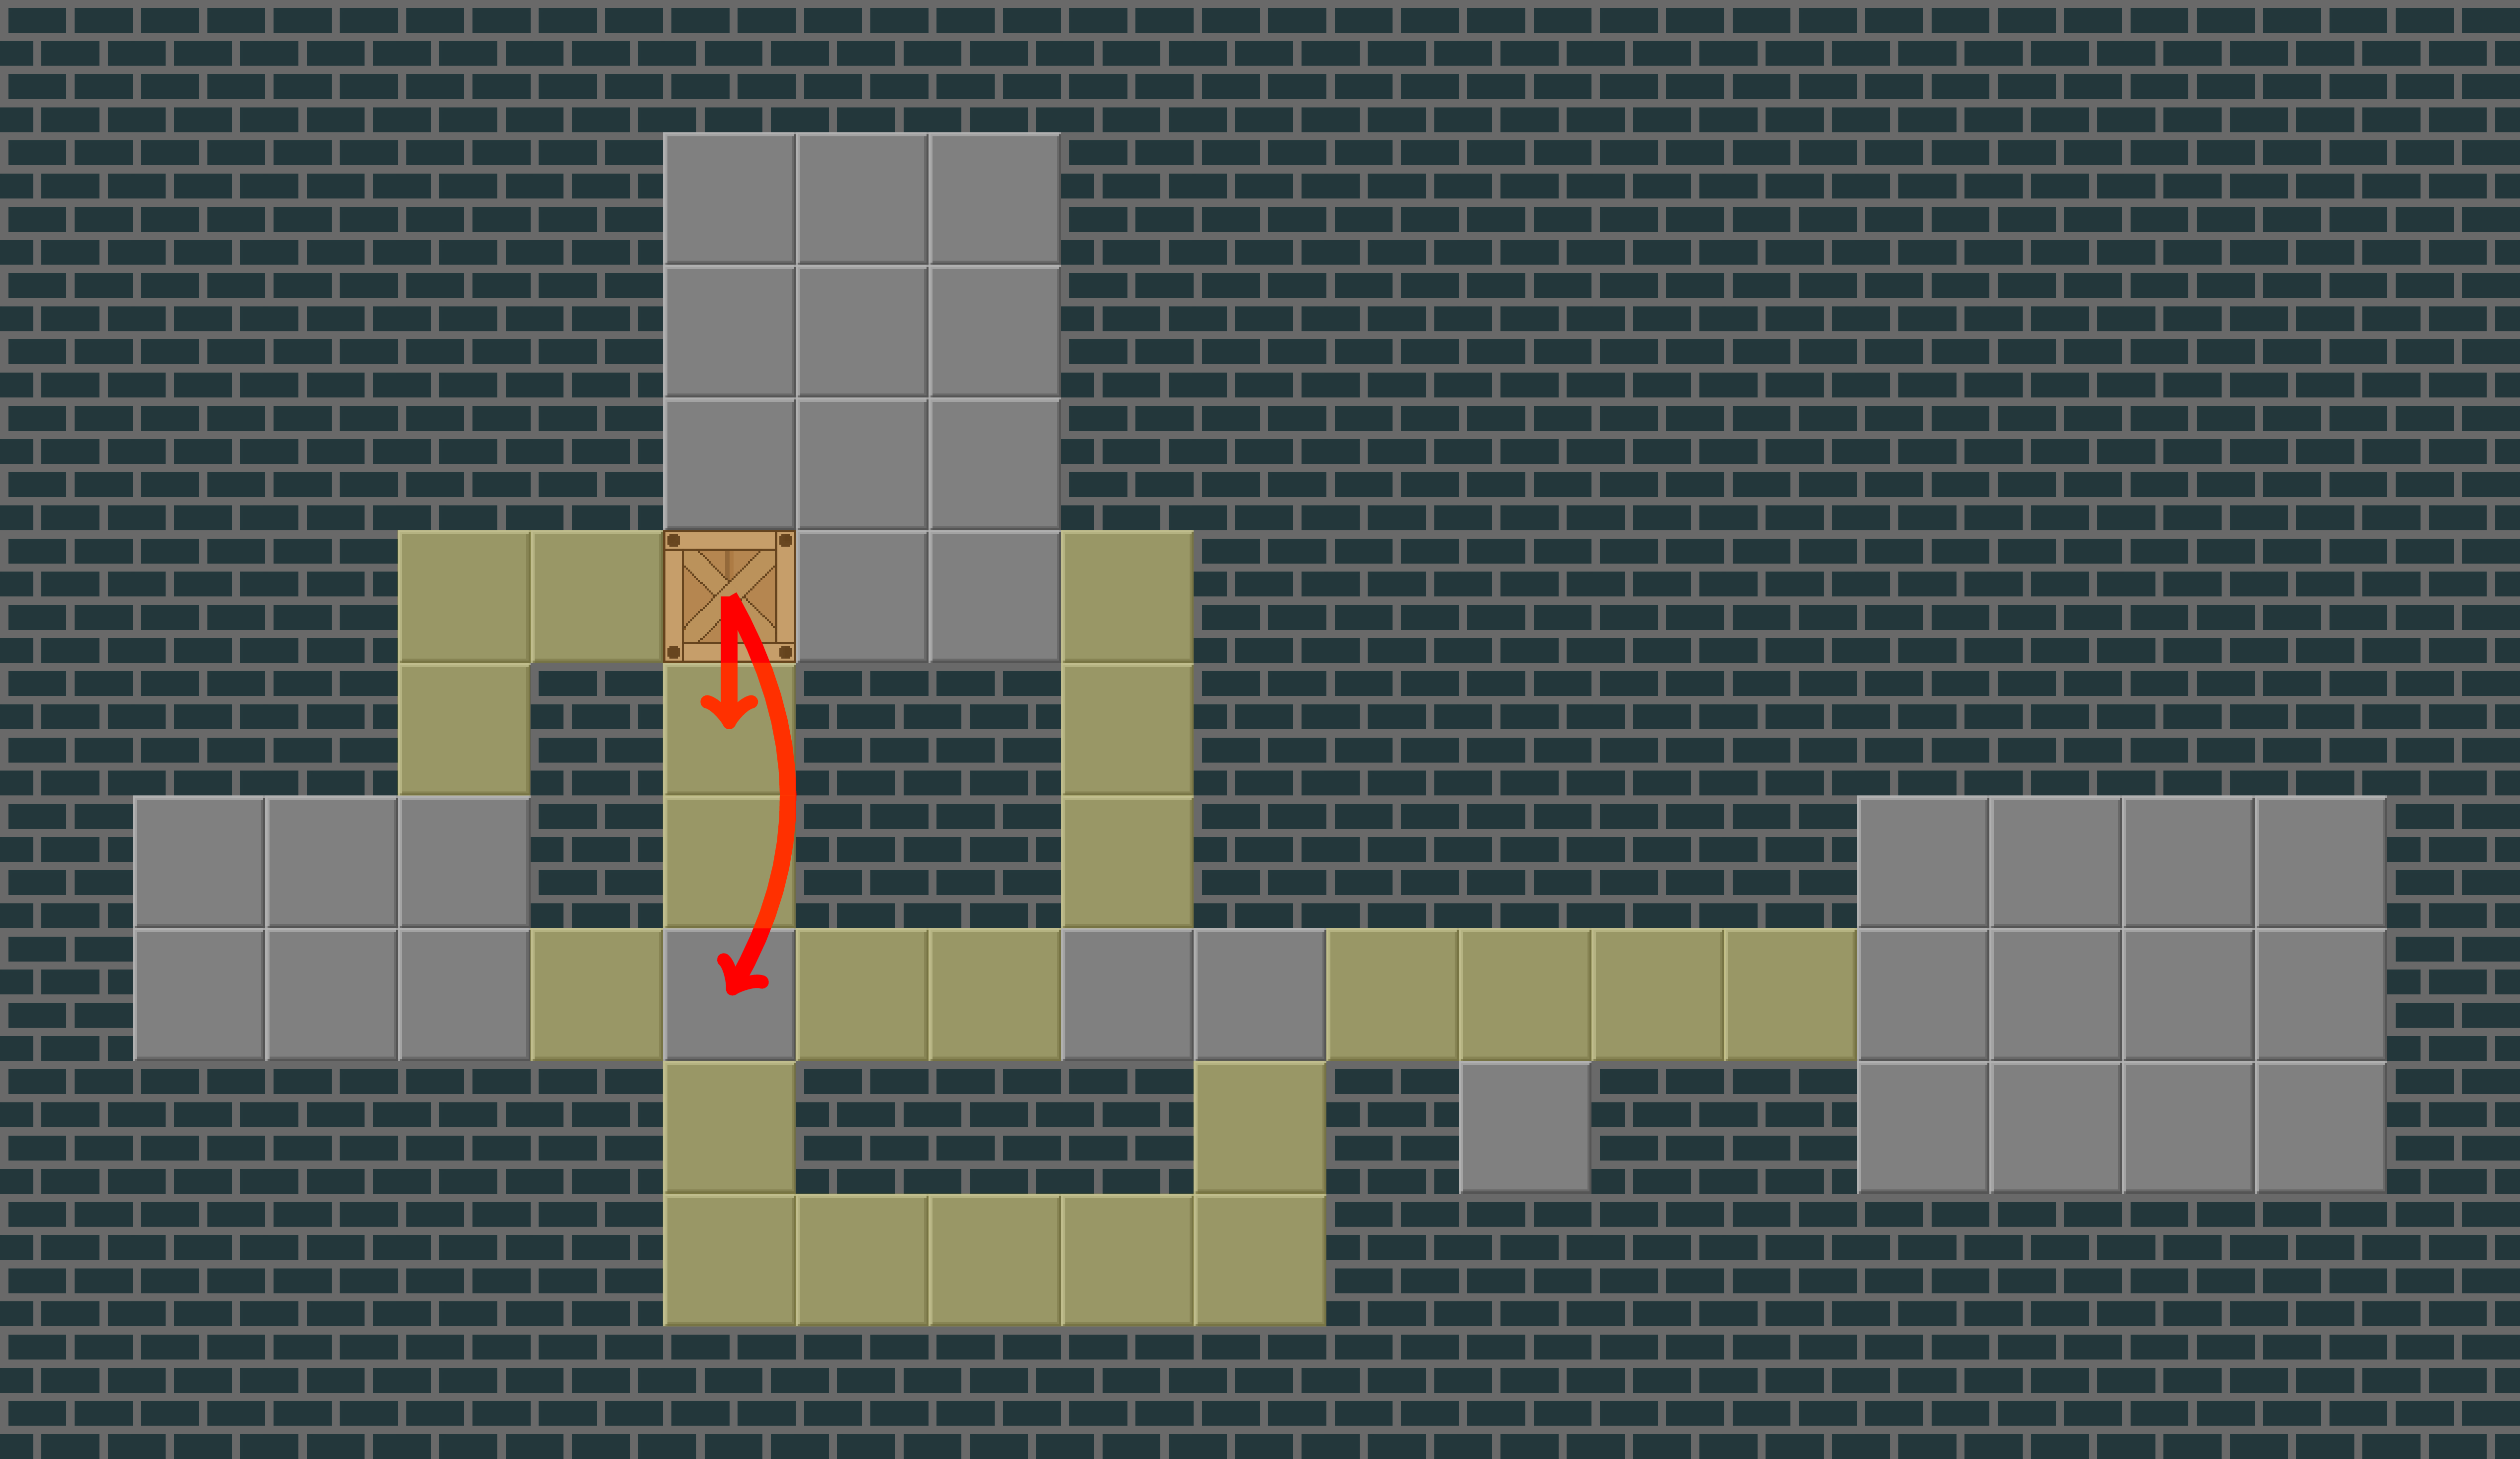
\includegraphics[width=\textwidth]{tunnels/tunnel_macro.png}
                }
                \only<3>{
                    \includegraphics[width=\textwidth]{tunnels/tunnel_macro_player_only.png}
                }
                \only<4>{
                    \includegraphics[width=\textwidth]{tunnels/tunnel_macro_oneway.png}
                }
                \only<5>{
                    \begin{minipage}{0.4\textwidth}
                         \includegraphics[width=\textwidth]{tunnels/straight.png}
                    \end{minipage}
                    \hfill
                    \begin{minipage}{0.4\textwidth}
                         \includegraphics[width=\textwidth]{tunnels/corner.png}
                    \end{minipage}
                }
            \end{frame}

            \begin{frame}{Calcul d'un ordre de rangement \textit{(packing order)}}
            \end{frame}

        \subsection{Analyse dynamique}

            \begin{frame}{Détection d'impasses \textit{(deadlocks)}}
                % Ajouter un exemple simple de deaedlock ?
                \begin{figure}
                    \centering
                    \subcaptionbox{\textit{Freeze deadlock n°1}} {
                        \includegraphics[width=0.3\textwidth]{freeze_deadlock/ex_1_dead.png}
                    }
                    \subcaptionbox{\textit{Freeze deadlock n°2}} {
                        \includegraphics[width=0.3\textwidth]{freeze_deadlock/ex_2_dead.png}
                    }
                    \subcaptionbox{\textit{PI Corral deadlock}} {
                        \includegraphics[width=0.3\textwidth]{pi_corral_deadlock_dead.png}
                    }
                \end{figure}
            \end{frame}

            \begin{frame}{Détection de \textit{freeze deadlocks}}
                \begin{figure}
                    \subcaptionbox{\textit{Règle n°1}} {
                        \includegraphics[width=0.3\textwidth]{freeze_deadlock/rule_1.png}
                    }
                    \subcaptionbox{\textit{Règle n°2}} {
                        \includegraphics[width=0.3\textwidth]{freeze_deadlock/rule_2.png}
                    }
                    \subcaptionbox{\textit{Règle n°3}} {
                        \includegraphics[width=0.3\textwidth]{freeze_deadlock/rule_3.png}
                    }
                \end{figure}
            \end{frame}

            \begin{frame}{Détection de \textit{freeze deadlocks}}
                \centering
                \begin{tikzpicture}
                    \node (start) {
                        \includegraphics[width=0.4\textwidth]{freeze_deadlock/ex_2_dead.png}
                    };
                    \node[visible on=<2-4>, right=of start] (first) {
                        \includegraphics[width=0.4\textwidth]{freeze_deadlock/ex_2_explanation_1.png}
                    };
                    \node[visible on=<3-4>, below=of first] (second) {
                        \includegraphics[width=0.4\textwidth]{freeze_deadlock/ex_2_explanation_2.png}
                    };
                    \node[visible on=<4>, left=of second] (third) {
                        \includegraphics[width=0.4\textwidth]{freeze_deadlock/ex_2_explanation_3.png}
                    };
                    % don't remove '0cm', otherwise tikz will place the text too below
                    \node [visible on=<4>, below=0cm of third.south] {Gelée!};

                    \draw[->, line width=\arrowwidth, visible on=<2-4>] (start.east)  -- (first.west);
                    \draw[->, line width=\arrowwidth, visible on=<3-4>] (first.south) -- (second.north);
                    \draw[->, line width=\arrowwidth, visible on=<4>] (second.west) -- (third.east);
                \end{tikzpicture}
            \end{frame}
            \begin{frame}{Détection de \textit{PI Corral deadlocks}}

            \end{frame}
            \begin{frame}{Table de \textit{deadlocks}}
                \only<1>{
                    \centering
                    \includegraphics[width=0.6\textwidth]{deadlock_table/init.png}
                }
                \only<2>{
                    \centering
                    \includegraphics[width=0.6\textwidth]{deadlock_table/new_deadlock.png}
                }
            \end{frame}

    \section{Recherche dirigée par une heuristique}
        \begin{frame}{Heuristique simple \textit{(Simple Lower Bound)}}

            \only<1>{

            }
        \end{frame}

        \begin{frame}{Heuristique gloutonne \textit{(Greedy Lower Bound)}}
        \end{frame}

    \section{Optimisations}
        \begin{frame}{}
        \end{frame}

    \section{Résultats}
\end{document}
